\subsection{The fundamental domain and the tessellation of the halfplane}

We have seen in Remark~\ref{rem_NatureMoebius} that the group of M�bius transformations $\PGL{\C}$ acts on $\EC$ in a very natural way if we consider its elements as meromorphic functions $\EC \to \EC$ and identify function composition as group operation. Clearly this group action is also given for any subgroup of $\PGL{\C}$ and in particular for the modular group. 

For the following it will be convenient to write modular transformations in matrix form and the elements $z \in \EC$ as quotients $z = u/v$ for suitable $u,v \in \C$ with at least one of them nonzero. A formal quotient $u/0$ will be identified with $\infty$. In this notation, for a modular transformation $A = \smallmat{a}{b}{c}{d} \in \PSL{\Z}$ and $u/v \in \EC$ the group action is given by
\begin{equation}
\label{eqn_ModGrpAction}
A \ \frac{u}{v} := \frac{a u + b v}{c u + d v}
\end{equation}
As usual, we call two points $z, w \in \EC$ \emph{equivalent}, if and only if there is a modular transformation $A \in \PSL{\Z}$ with $A z = w$ and we write  $z \sim w$. The equivalence class (\emph{orbit}) of a point $u/v \in \EC$ is written as $[u/v]_\sim \in \EC/\sim$ and consists of all points
\begin{equation*}
\frac{a u + b v}{c u + d v} \in \EC, \quad \text{where }{\mat{a}{b}{c}{d} \in \PSL{\Z}}
\end{equation*}
runs over all elements of the modular group. We now wish to find a system of representatives for $\EC/\sim$, \ie we want to pick exactly one point $u_0/v_0$ out of each $[u/v]_\sim$ as a representative. One approach for this could be to fix $u,v \in \C$, not both zero, then to choose from the set
\begin{equation*}
L_{u,v} := \setdefsz{\bigg}{\cvec{a u + b v}{c u + d v} \in \C^2}{\mat{a}{b}{c}{d} \in \PSL{\Z}}
\end{equation*}
one vector $(u_0, v_0)$ with minimal $\eucnorm{\cdot}$-norm and to declare $u_0/v_0$ as the representative for $[u/v]_\sim$. The problem with this is that in general $L_{u,v}$ may contain vectors of arbitrary small norm. Thus the existence of such a vector $(u_0, v_0)$ is not guaranteed. 

\begin{figure}
\centering
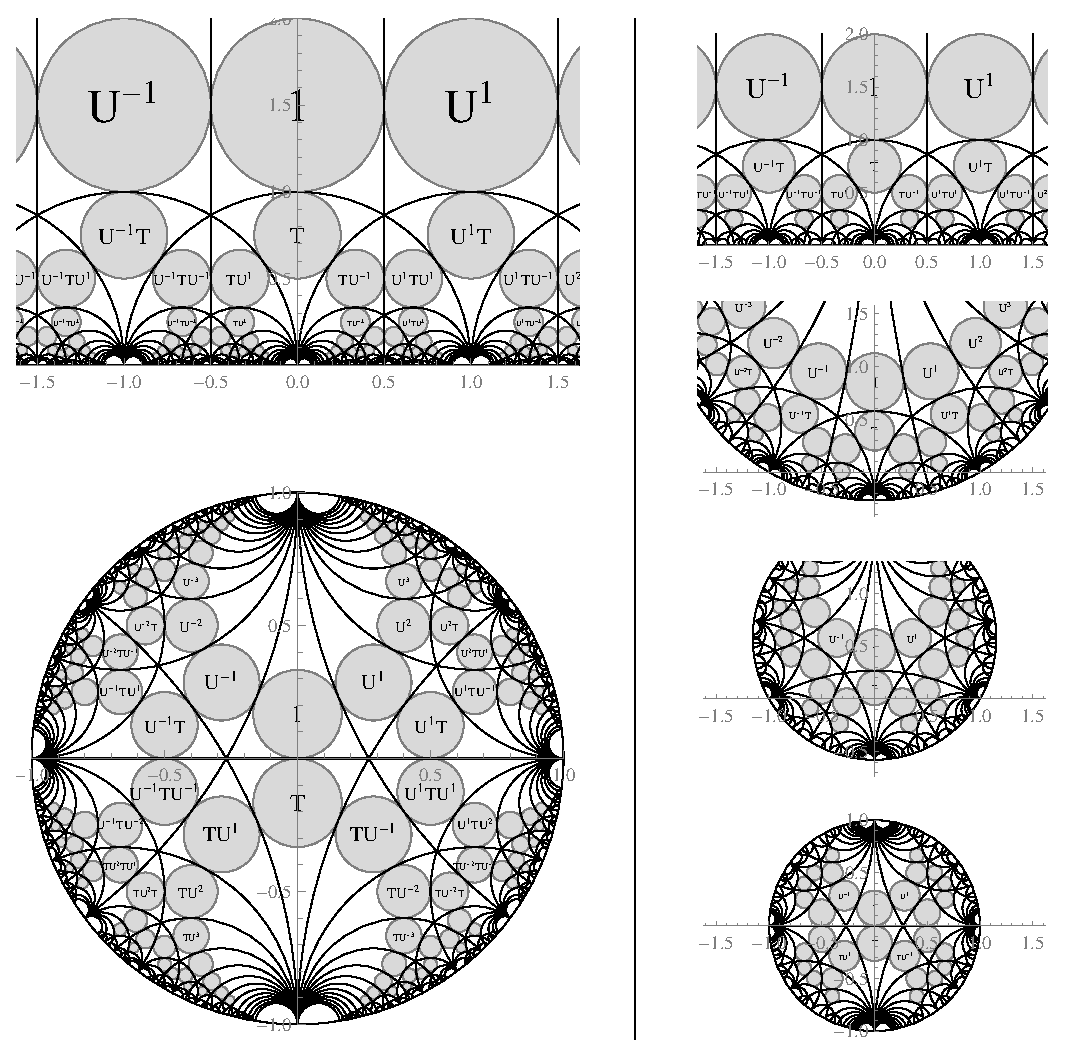
\includegraphics[width=\textwidth]{figures/modular-tiling-1}
\caption{The tessellation of the upper halfplane.}
\label{fig_ModularTiling}
\end{figure}

\begin{figure}
\centering
\includegraphics[width=0.8\textwidth]{figures/modular-tiling-exp-fan}
\caption{The tessellation under the transformation $z \mapsto \exp(2 \pi \ii z)$.}
\label{fig_ModularTilingExpFan}
\end{figure}

\begin{figure}
\centering
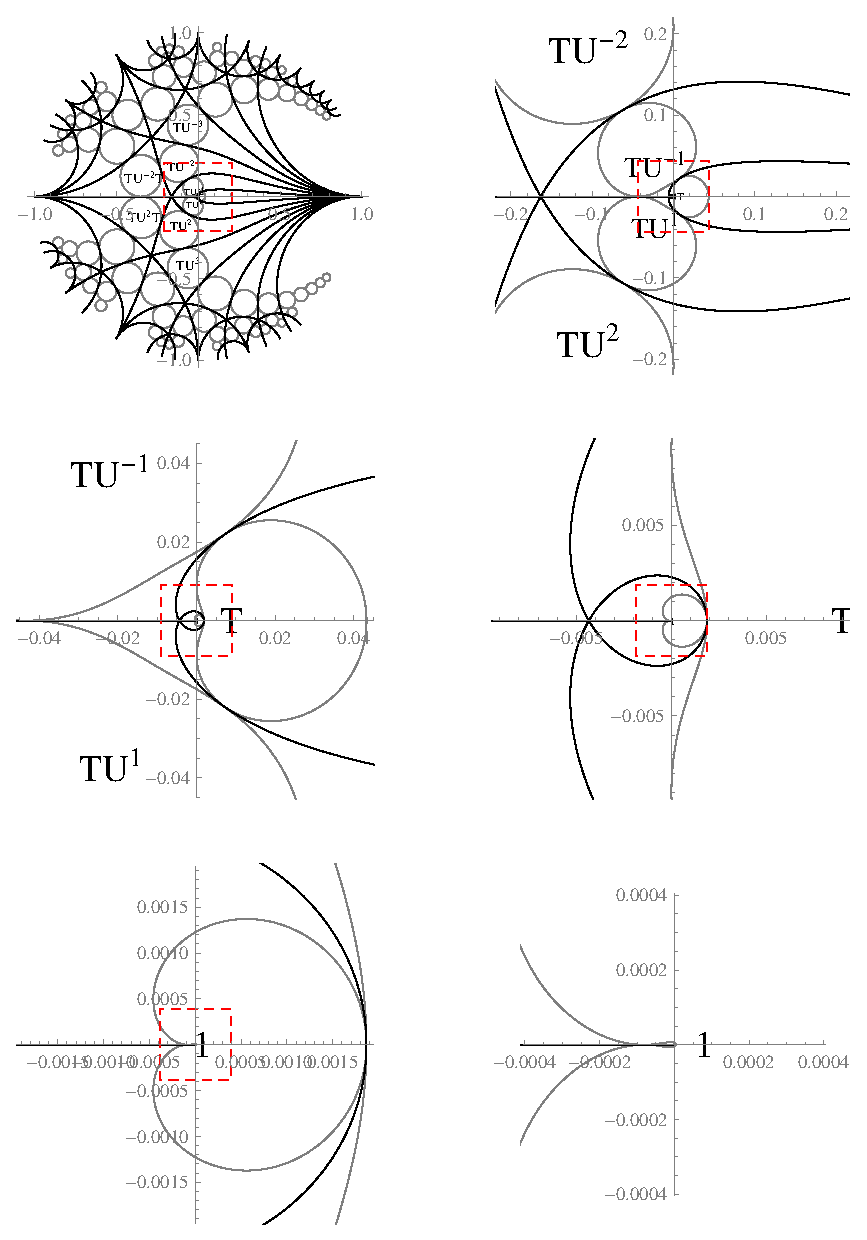
\includegraphics[width=0.8\textwidth]{figures/modular-tiling-exp-zoom}
\caption{The image of the modular tiling under the map $z \mapsto \exp(2 \pi \ii z)$ in the neighborhood of $\infty$.}
\label{fig_ModularTilingExpZoom}
\end{figure}

\todo{25}{Definition, description and figures}
